\documentclass[12pt]{article}%
% Used for centring the title
\usepackage{titlesec}
\titleformat{\section}[block]{\Large\bfseries\filcenter}{}{1em}{}

% Packages
\usepackage{amsfonts}
\usepackage{fancyhdr}
\usepackage{comment}
\usepackage[a4paper, top=2.5cm, bottom=2.5cm, left=2.2cm, right=2.2cm]%
{geometry}
\usepackage{times}
\usepackage{amsmath}
\usepackage{changepage}
\usepackage{amssymb}
\usepackage{graphicx}%
\usepackage{xcolor}
\usepackage{breqn}

% Theorem Formats
\setcounter{MaxMatrixCols}{30}
\newtheorem{theorem}{Theorem}
\newtheorem{acknowledgement}[theorem]{Acknowledgement}
\newtheorem{algorithm}[theorem]{Algorithm}
\newtheorem{axiom}{Axiom}
\newtheorem{case}[theorem]{Case}
\newtheorem{claim}[theorem]{Claim}
\newtheorem{conclusion}[theorem]{Conclusion}
\newtheorem{conjecture}[theorem]{Conjecture}
\newtheorem{corollary}[theorem]{Corollary}
\newtheorem{criterion}[theorem]{Criterion}
\newtheorem{definition}[theorem]{Definition}
\newtheorem{example}[theorem]{Example}
\newtheorem{exercise}[theorem]{Exercise}
\newtheorem{lemma}[theorem]{Lemma}
\newtheorem{notation}[theorem]{Notation}
\newtheorem{problem}[theorem]{Problem}
\newtheorem{proposition}[theorem]{Proposition}
\newtheorem{remark}[theorem]{Remark}
\newtheorem{solution}[theorem]{Solution}
\newtheorem{summary}[theorem]{Summary}
\newenvironment{proof}[1][Proof]{\textbf{#1.} }{\ \rule{0.5em}{0.5em}}

% new commands for readability
\newcommand{\C}{\mathbb{C}}
\newcommand{\F}{\mathbb{F}}
\newcommand{\N}{\mathbb{N}}
\newcommand{\Q}{\mathbb{Q}}
\newcommand{\R}{\mathbb{R}}
\newcommand{\Z}{\mathbb{Z}}
\newcommand{\Mod}[1]{\ (\mathrm{mod}\ #1)}
\newcommand{\rpm}{\raisebox{.2ex}{$\scriptstyle\pm$}}

\begin{document}

% Title
\title{Assignment 2}
\author{Robert Lech}
\date{\today}
\maketitle
\section*{Chapter 3}

\subsection*{Question 13}

Show that $A*B$ is a free group if and only if $A$ and $B$ are free.\\

$(\Rightarrow)$ Assume $A*B$ is a free group. We'd like to show that $A$ and $B$ are free. Firstly, we note that $A$ and $B$ are definitely subgroups of $A*B$. This can be seen in Corollary 3.27 that states that groups $A$ and $B$ inject into $A*B$. Therefore, we can use Corollary 3.23 (Nielsen-Schreier) to say that the subgroups $A$ and $B$ are themselves free.\\

$(\Leftarrow)$ Assume $A$ and $B$ are free groups. Then there exist bases $S_A$ and $S_B$ such that $A=<S_A>$ and $B=<S_B>$ and no non-trivial, freely reduced word represents the identity $1_A$ and $1_B$, respectively. We want to show $A*B$ is free. That is, we want to show there exists a basis $S_{A*B}$ such that $<S_{A*B}>=A*B$ and no non-trivial freely reduced word represents the identity $1_{A*B}$, respectively.

Therefore, we can let $S_{A*B}=S_A \cup S_B$. We also note that, without loss of generality, every word in $A*B$ is of the form $w=a_{1}b_{1}a_{2}b_{2}\ldots a_{n}b_{n}$ for some $a_i\in A$ and $b_i\in B$. Two things should be noted: 

\begin{enumerate}
\item For all $i\in {1, 2, \ldots n}$, $b_{i-1} \neq a_i \neq b_i$ and $b_{i-1} \neq a_i^{-1} \neq b_i$ (as they were from different groups)
\item For all $i\in {1, 2, \ldots n}$, $a_i$ and $b_i$ are themselves non-trivial, freely reduced words (as they are from free groups).
\end{enumerate}

Therefore, this word cannot freely reduce to $1_{A*B}$. Therefore, $A*B$ must be free.
\subsection*{Question 14}

Let $\F_2$ be a free group with basis $\{x,y\}$, and let $K$
 be the kernel of the homomorphism $\phi:\F_2\rightarrow \Z_3$ induced by $\phi(x)=\phi(y)=1$.

% Taken from: https://www.sharelatex.com/learn/Lists
\renewcommand{\labelenumi}{\alph{enumi}}
\begin{enumerate}
  \item Find the fundamental domain for the action of $K$ on the Cayley graph of $\F_2$.
\end{enumerate}

\textbf{How does $K$ look}

Firstly, from computation, we see that, in order of lengths, they are: . 
\begin{align*}
K
&=\{e\} \\
&\cup\{xy^{-1}, x^{-1}y, (xy^{-1})^{-1}, (x^{-1}y)^{-1}\} \\
&\cup\{xxx,xxy,xyx,xyy,yxx,yxy,yyx,yyy, \\
&(xxx)^{-1},(xxy)^{-1},(xyx)^{-1},(xyy)^{-1},(yxx)^{-1},(yxy)^{-1},(yyx)^{-1},(yyy)^{-1}\} \\
&\cup \ldots
\end{align*}


Therefore, we can think of $K$ as the words with exponents adding up to $0 \Mod{n}$. More formally, $K=\{a_{1}^{\varepsilon_1}a_{2}^{\varepsilon_1}\ldots a_{n}^{\varepsilon_1} | a_i=w\in \F_2, \varepsilon_i\in \{-1, 1\}, \sum_{i=1}^{n} \varepsilon_i \equiv 0 \Mod{n}\}$. \\

\textbf{The Cayley Graph for $\F_2$ and the Fundamental Domain for $K$}

As seen in the book in Figure 3.1 and as claimed in Corollary 3.4 on page on page 56, the free group $\F_2$ can be viewed as a group of symmetries of $\mathcal{T}_4$. The fundamental domain, $\mathcal{F}$, that I'm choosing for $K$, will initially consist of vertex $e$. To know what other vertices get added to $\mathcal{F}$, we can note that for every word $k\in K$ and for every $w\not\in K$, it can be shown that $wk\not\in K$. That is, $wk$ is not a word with exponents adding up to $0\Mod{k}$. Therefore vertices $x$ and $x^2$, along with the edges between ($e$ and $x$) and ($x$ and $x^2$) can be added to $\mathcal{F}$. Lastly, adding the half-edges connected to the three vertices gives us $\mathcal{F}$. This can all be seen in Figure \ref{fig:fun_domain_of_K} below.

\begin{figure}[ht]
    \centering
    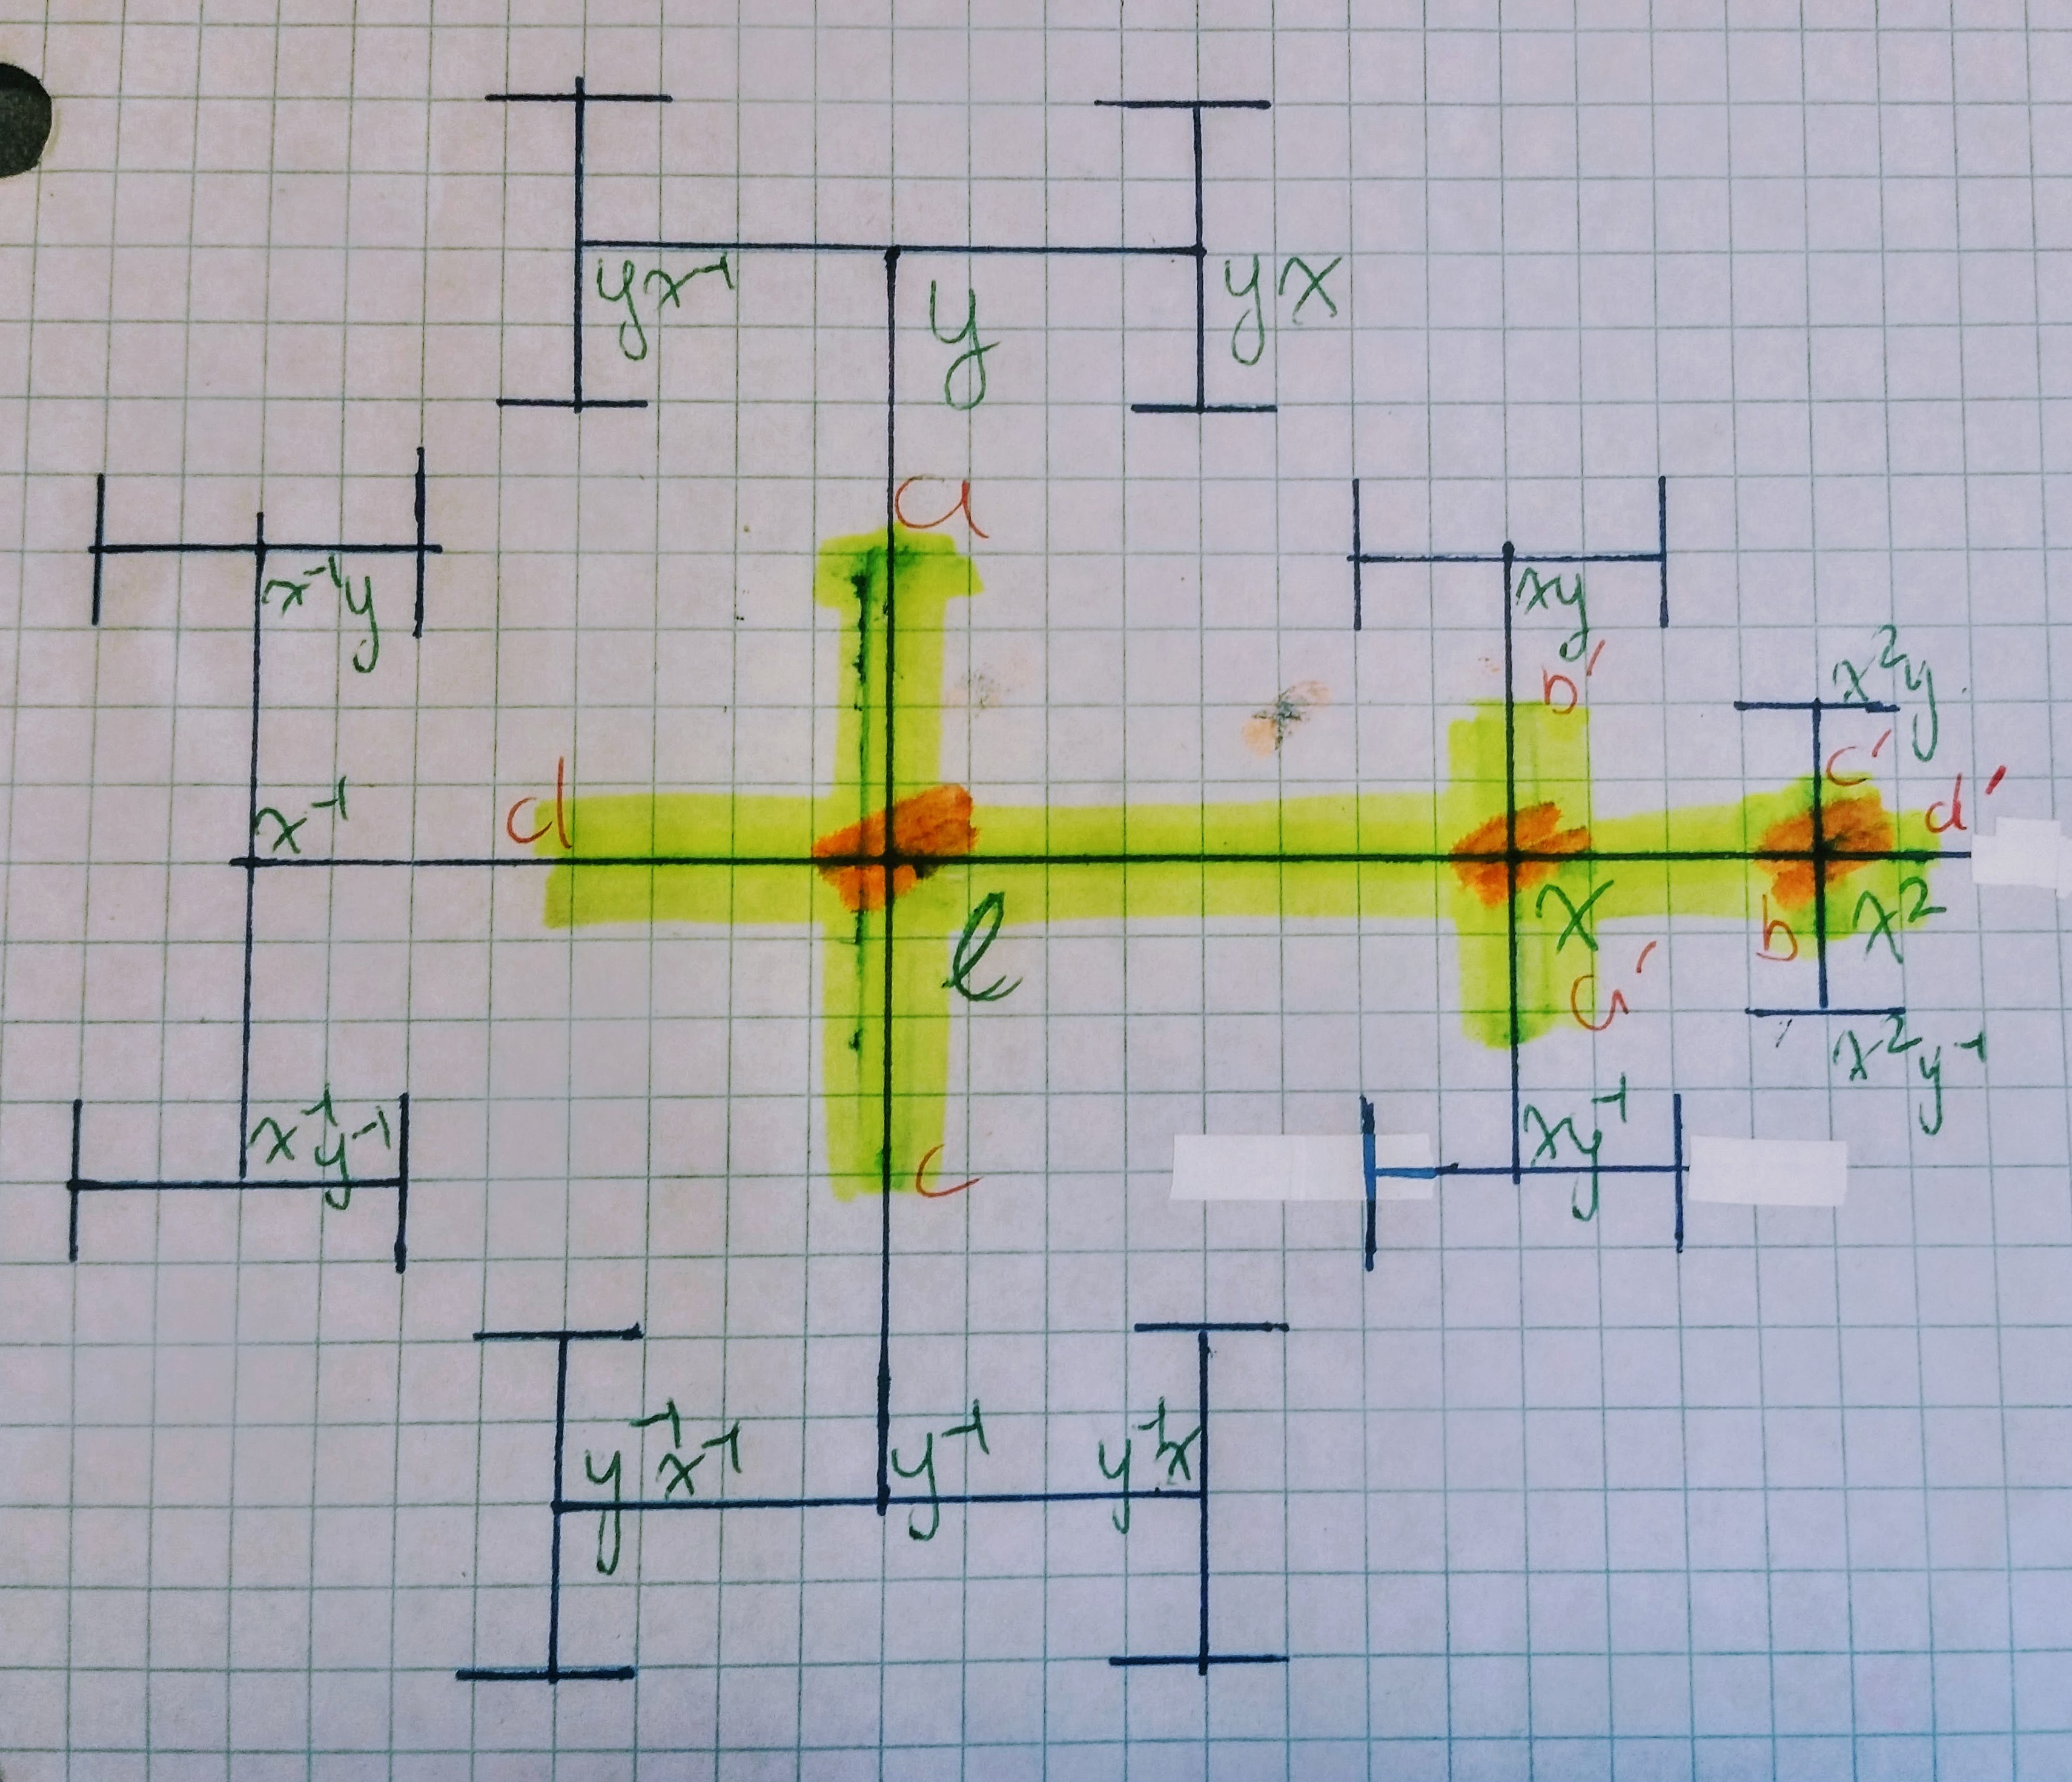
\includegraphics[width=1.0\textwidth]{images/fundamental_domain_for_K.jpg}
    \caption{The Cayley graph for $\F_2$ and the fundamental domain, $\mathcal{F}$, for $K$. Also listed are labels for endpoints of half-edges attached to vertices in $\mathcal{F}$.}
    \label{fig:fun_domain_of_K}
\end{figure}

\begin{enumerate}
  \setcounter{enumi}{1}
  \item Find a basis $S$ for the kernel $K$.
\end{enumerate}

Using Figure \ref{fig:fun_domain_of_K} as a visual aid, we see there are eight half-edges in $\mathcal{F}$. This implies there should be four elements in our basis $S$ such that $S^{\rpm}=\left\{g\in K | g\mathcal{F} \cap \mathcal{F} \neq \emptyset \right\}$. These should be the elements that map ends of half-edges in $\mathcal{F}$ to ends of half-edges $\mathcal{F}$.  Good ones to start with are the words in the kernel that have `minimal' length. Apart from the identity, these are the words listed at the beginning of this question. Start by adding $xy^{-1}$ (which can map point $a$ to $a'$) and $x^{-1}y$ (which can map point $b$ to $b'$) to $S$ as they are not inverses of each other. We proceed by adding $xxx$ (which can map point $c$ to $c'$) to $S$. We also note these three words generate $xyy, yyx,$ and $yyy$). We finally add $xyx$ (which can map point $d$ to $d'$) to $S$. We also note that $xy^{-1}, x^{-1}y,$ and $xyx$  generate the remaining words $xxy, yxx,$ and $yxy$). 

At this point, all words of length 2 and 3 can be generated. Therefore, the basis for $\mathcal{F}$ is $S=\left\{xy^{-1}, x^{-1}y, xxx, xyx\right\}$.

\subsection*{Question 18}

Let $A$ and $B$ be non-trivial groups. Prove that the centre of $A*B$ is trivial. \\

Let $A$ and $B$ be non-trivial groups. Denote the centre of $G$ as $Z(A*B)=\{ w \in A*B | wx=xw, \forall x \in A*B \}$. Clearly the identity is in $Z(A*B)$ since the identity must commute with every element in a group. However, to prove that no other elements in $A*B$ are in $Z(A*B)$ , we'll do a proof by contradiction. That is, we'll suppose there exists a $w\in Z(A*B)$ such that $w \neq 1_{A*B}$. Then this $w$ commutes with every word $x \in A*B$. We'll show this is impossible by finding a word, in every case, that cannot possibly commute with $w$.

\textbf{Case 1}: Suppose $w=a_{1}b_{1}a_{2}b_{2}\ldots a_{n}b_{n}$, where $a_1,a_2,\ldots ,a_n, b_1,b_2,\ldots b_n$ are not the identity. Then let $x=a_1$ and look at the word $wxw^{-1}x^{-1}$. We see that:

\begin{dmath}
wxw^{-1}x^{-1}=(a_{1}b_{1}a_{2}b_{2}\ldots a_{n}b_{n})(a_{1})(b_{n}^{-1}a_{n}^{-1}\ldots b_{2}^{-1}a_{2}^{-1}b_{1}^{-1}a_{1}^{-1})(a_{1}^{-1}) \neq 1
\end{dmath}

as it doesn't freely reduce.

\textbf{Case 2}: Suppose $w=b_{1}a_{1}b_{2}a_{2}\ldots b_{n}a_{n}$, where $a_1,a_2,\ldots ,a_n, b_1,b_2,\ldots b_n$ are not the identity. Then let $x=b_1$ and refer to \textbf{Case 1} for the proof structure. 

\textbf{Case 3}: Suppose $w=a_{1}b_{1}a_{2}b_{2}\ldots a_{n}$, where $a_1,a_2,\ldots ,a_n, b_1,b_2,\ldots b_{n-1}$ are not the identity. Then let $x=b_{n-1}$ and look at the word $wxw^{-1}x^{-1}$. We see that:

\begin{dmath}
wxw^{-1}x^{-1}=(a_{1}b_{1}a_{2}b_{2}\ldots a_{n})(b_{n-1})(a_{n}^{-1}\ldots b_{2}^{-1}a_{2}^{-1}b_{1}^{-1}a_{1}^{-1})(b_{n-1}^{-1}) \neq 1
\end{dmath}

as it doesn't freely reduce.

\textbf{Case 4}: Suppose $w=b_{1}a_{1}b_{2}a_{2}\ldots b_{n}$, where $a_1,a_2,\ldots ,a_{n-1}, b_1,b_2,\ldots b_n$ are not the identity. Then let $x=a_{n-1}$ and refer to \textbf{Case 3} for the proof structure. 

Since these 4 cases represent every non-trivial, reduced word in $A*B$ , we see that that $Z(A*B)$ must be trivial.

\section*{Chapter 4}

\subsection*{Question 7}

Prove that the smallest normal subgroup of $BS(1, 2)$ that contains $b$ is isomorphic to the dyadic rationals.\\

\textbf{Step 1: Find the smallest normal subgroup $BS(1,2)$ containing $b$.}

We'll first note what facts we'll need for this problem. Firstly, we note that $BS(1,2)=<a,b|aba^1=b^2>$ , where  $a(x)=2x$ and $b(x)=x+1$.  From Proposition 4.1 on page 102 in the book, we know that: 
\begin{equation}
BS(1,2)=\left\{g(x) | g(x)=\frac{2^{n+k}x+m}{2^k}, \forall k, m, n \in \Z \right\}
\end{equation}
Now, the question is asking us for the smallest subgroup of $BS(1,2)$ that contains $b$. There is a fact that the conjugate/normal closure of a generating set $S$ is precisely this. The normal closure is defined as $S^G=\left\{g^{-1}sg|\forall g\in G, s\in S\right\}$. Since $S=\{b\}$, this simplifies to $S^G=\left\{g^{-1}bg|\forall g\in G\right\}$. Therefore, for some $n$, and for some $g(x)$, we can compute $g^{-1}(b(g(x)))$. Below, we see it simplifies to:

\begin{align*}
g^{-1}(b(g(x)))
&= g^{-1}\left(b\left(\frac{2^{n+k}x+m}{2^k}\right)\right) \\
&= g^{-1}\left(\frac{2^{n+k}x+m}{2^k}+1\right) \\
&= g^{-1}\left(\frac{2^{n+k}x+m+2^k}{2^k}\right) \\
&= \frac{2^k\left(\frac{2^{n+k}x+m+2^k}{2^k}\right)-m}{2^{n+k}} \\
&= \frac{2^{n+k}x+m+2^k-m}{2^{n+k}} \\
&= \frac{2^{n+k}x+2^k}{2^{n+k}} \\
&= x+\frac{1}{2^{n}}
\end{align*}

Therefore, $S^G=\left\{g(x)|g(x)=x+\frac{1}{2^{n}}, \forall n\in \Z\right\}$.\\

\textbf{Step 2: Show $S^G\simeq$  the group $\left(\Z\left[\frac{1}{2}\right],+\right)$}

\textbf{Step 2a: Find $\phi$}

To see this, first denote $\Z\left[\frac{1}{2}\right]=\{ \frac{i}{2^j} | i \in \Z, j \in \N \}$. Then to define our mapping $\phi:S^G \rightarrow \Z\left[\frac{1}{2}\right]$ is better explained with an example. Suppose we'd like to find some function in $S^G$  that maps to some element in the group $\left(\Z\left[\frac{1}{2}\right],+\right)$, say $\frac{3}{2^2}$. Then we note that:
\begin{align*}
g_2^3(x)
&=g_2^2(x+\frac{1}{2^2})\\
&=g_2(x+\frac{1}{2^2}+\frac{1}{2^2})\\
&=g_2(x+\frac{2}{2^2})\\
&=x+\frac{1}{2^2}+\frac{2}{2^2}\\
&=x+\frac{3}{2^2}
\end{align*}

Therefore, we should let $\phi$ be the map that takes the dyadic constant term in  $g_2^3(x)$ to the corresponding element in the group $\left(\Z\left[\frac{1}{2}\right],+\right)$. More formally, we're saying that $\phi(g_j^i(x))=\frac{i}{2^j}$. 

\textbf{Step 2b: Show $\phi$ is a bijection}

It should be quite clear this is mapping is onto from based on the construction. Moreover, it's quite easy to see that the mapping is one-to-one. Suppose $g,h$ are such that $\phi(g_{j_1}^{i_1}(x))=\phi(g_{j_2}^{i_2}(x))$ for some $i_1,i_2,j_1,j_2$. Then we want to show $g_{j_1}^{i_1}(x)=g_{j_2}^{i_2}(x)$. Therefore, we can assume that $\frac{i_1}{2^{j_1}}=\frac{i_2}{2^{j_2}}$. Adding $x$ to both sides gives us  $x+\frac{i_1}{2^{j_1}}=x+\frac{i_2}{2^{j_2}}\Leftrightarrow g_{j_1}^{i_1}(x)=g_{j_2}^{i_2}(x)$. Therefore, $\phi$ is a bijection. 

\textbf{Step 2c: Show $\phi$ is a homomorphism}

To show this is a group homomorphism, we note that if we take two functions $g_{j_1}^{i_1}, g_{j_2}^{i_2} \in S^G$, then we see that:

\begin{align*}
\phi\left(g_{j_2}^{i_2} \circ g_{j_1}^{i_1}\right)
&=\phi \left(g_{j_2}^{i_2}\left(x+\frac{i_{1}}{2^{j_1}}\right)\right) \\
&=\phi\left(x+\frac{i_{2}}{2^{j_2}}+\frac{i_{1}}{2^{j_1}}\right) \\
&=\frac{i_{2}}{2^{j_2}}+\frac{i_{1}}{2^{j_1}}
\end{align*}
Performing the mapping first, we see that:
\begin{align*}
\phi\left(g_{j_2}^{i_2}\right)\phi\left(g_{j_1}^{i_1}\right)
&=\phi \left(x+\frac{i_{2}}{2^{j_2}}\right)\phi \left(x+\frac{i_{1}}{2^{j_1}}\right) \\
&=\left(\frac{i_{2}}{2^{j_2}}\right) + \left(\frac{i_{1}}{2^{j_1}}\right) \\
&=\frac{i_{2}}{2^{j_2}}+\frac{i_{1}}{2^{j_1}}
\end{align*}
Since $\phi\left(g_{j_2}^{i_2}\right)\phi\left(g_{j_1}^{i_1}\right)=\phi\left(g_{j_2}^{i_2} \circ g_{j_1}^{i_1}\right)$, we see that $\phi$ is a group homomorphism, and so $\phi$ is a group isomorphism as well. \\

This shows that $S^G\simeq \Z\left[\frac{1}{2}\right]$.

\end{document}
